\documentclass[10pt]{article}
\usepackage[OT1]{fontenc}
\usepackage[utf8]{inputenc}
\bibliographystyle{plain}

\usepackage[ruled,vlined]{algorithm2e}
\usepackage{amsmath}
\usepackage{amssymb}
\usepackage{gensymb}
\usepackage{mathrsfs}
\usepackage{mathtools}
\usepackage{esint}
\usepackage{braket}
\usepackage{array}
\usepackage{epsfig}
\usepackage{hyperref}
\renewcommand{\baselinestretch}{1.2}
\setlength{\textheight}{9in}
\setlength{\textwidth}{6.5in}
\setlength{\headheight}{0in}
\setlength{\headsep}{0in}
\setlength{\topmargin}{0in}
\setlength{\oddsidemargin}{0in}
\setlength{\evensidemargin}{0in}
\setlength{\parindent}{.3in}


\DeclarePairedDelimiter{\abs}{\lvert}{\rvert} %create the norm sign as symbol
\DeclarePairedDelimiter{\norm}{\lVert}{\rVert} %create the norm sign as symbol

% swap definition of \abs* and \norm* with \abs and \norm
% to scale delimiters without needing to type *
\makeatletter
\let\oldabs\abs
\def\abs{\@ifstar{\oldabs}{\oldabs*}}
\let\oldnorm\norm
\def\norm{\@ifstar{\oldnorm}{\oldnorm*}}
\makeatother

%custom commands here
% \newcommand{\new_command_name}{replacement text}


\begin{document}
\begin{center}
    \textbf{\large Beyond mean field solutions to the lattice mixture model} \\
    Gabriel Brown
\end{center}

%OUTLINE
% statistical thermodynamics review?
% lattice model
% - coordination number, dimension
% - energy of interaction
% - simple results and equations
% - mean field approximation and internal energy formula
% computational approach
% some extremum bounds

\section{Introduction and motivation}
The approximate Bragg-Williams solution to the binary lattice mixture model is both simple and useful, though one must take to stay within it's domain of applicability.
Direct consequences of this approximate model include the regular solution model, which itself provides an entry point to the study of phase separation \cite{dill}.
Therefore, a more accurate solution to the binary lattice mixture model could provide better models for physical phenomena in statistical and classical thermodynamics.
In the present paper we venture to create such an improved model via semi-emperical means.
An algorithm, called the ``Metropolis algorithm for lattice mixtures'' is developed and used to generate a data set over the parameter space of variables on which the internal energy per site $\hat{U}$ [eV site$^{-1}$] depends.
Using this data set together with physical insights into the data and physical and symmetry constraints on the functinal form of $U$, an emperical form is proposed and numerically fit.


\section{Lattice model of a mixture} 

\subsection{Basics}
A mixture of two condensed (liquid or solid) phases $A$ and $B$ may be crudely described by a single-degree-of-freedom-per-site lattice model with uniform coordination number $z$, meaning that each lattice site has $z$ nearest neighbors. \footnote{The present model formulation of a mixture on a lattice follows closely to \cite{dill}, with minor modifications including my own motivations and explanations.} 
Restricting the energetic interactions to nearest neighbor pairwise, there are three energetic constants for $A-A$, $B-B$, and $A-B$ interactions, respectively: $w_{AA}, \; w_{BB}, \; w_{AB}$, which may be generically positive, negative, or zero.
Let $W$ represent a realization or configuration of the lattice, uniquely specifying the occupation of each site as $A$ or $B$.
The total internal energy $U$ of such a configuration is then given by
\begin{align}
    U(W) = m_{AA} w_{AA} + m_{BB} w_{BB} + m_{AB} w_{AB}
\end{align}
where $m_{XY}$ is the number of $X-Y$ interactions in the system.
Restricting to finite periodic lattice of $N$ total sites with $N_A$ $A$ sites and $N_B$ $B$ sites (uniquely defining a $B$ volume fraction $x = N_B / N$), one can further define the $m_{XY}$s.
Since each pairwise interaction involved two sites, the total number of interactions for a periodic lattice with $N$ sites and coordination $z$ is
\begin{align}
    m_{AA} + m_{BB} + m_{AB} = \frac{z N}{2} = \frac{z}{2} \left( N_A + N_B \right),
\end{align}
further,
\begin{align}
    \frac{z N_A}{2} = m_{AA} + \frac{m_{AB}}{2}, \quad\quad
    \frac{z N_B}{2} = m_{BB} + \frac{m_{AB}}{2}.
\end{align}
With $N$ and $x=N_B/N$ (equivalently $N_A$ and $N_B$) being known system constants, this model is nearly analytical apart from the unknown value of $m_{AB}$. \footnote{Realistic physical systems are often so large that it is more convenient to work in terms of densities like $N/V$, but since we will be interacting intimately with the lattice description, we maintain use of $N$ directly.} \footnote{One could also treat $m_{AA}$ or $m_{BB}$ as unknowns, the three $m_{X}$s are algebraically related such that one of the three uniquely defines the others.}

\subsection{Approximate solution}
To keep such a lattice model analytical, we use the Bragg-Williams mean field approximation, which posits that the $A$ and $B$ sites are randomly distributed throughout the lattice \cite{flory}.
One can then approximate that $A$ sites have on average $z N_B / N$ neighboring $B$ sites, and the corresponding approximation for $m_{AB}$ is
\begin{equation}
    m_{AB} \approx \frac{z N_A N_B}{N} = z N (1-x) x.
\end{equation}
The standard way of writing the total energy of this model is
\begin{align}
    U &=
    \frac{z w_{AA}}{2} N_A +
    \frac{z w_{BB}}{2} N_B +
    k_B T \chi_{AB} \frac{N_A N_B}{N}, \\
    \chi_{AB} &=
    \frac{z}{k_B T} \left( w_{AB} - \frac{w_{AA} + w_{BB}}{2} \right)
    \label{eqn:BW_solution}
\end{align}
where $\chi_{AB}$ is the dimensionless ``exchange parameter''. \footnote{Admittedly, I don't see the utility in artificially introducing temperature dependence to a temperature-independent model via $\chi_{AB}$, but I believe the dimensionless parameter does have some merit for extracting properties from experiment.}
The formula for average energy $\hat{U}=U/N$ per site is then
\begin{align}
    \hat{U} &=
    \frac{z w_{AA}}{2} (1-x) +
    \frac{z w_{BB}}{2} x +
    k_B T \chi_{AB} (1-x) x
\end{align}
which is useful for working with lattices of varying sizes.

We finish the introduction of the lattice model and mean field approximation by noting the possible errors associated with the Bragg-Williams approximation.
Addressing these completely requires a bit of statistical thermodynamics.
The internal energy of a system in a given macrostate (in this case given by system size $N$ and $B$ volume fraction $x$) generically depends on the energies of all the possible microstates $W_i$. \footnote{As an example, for a 1-D system of a binary mixture of macrostate $N=3$ and $x=1/3$ the possible microstates are $[A,A,B],\; [A,B,A],\; [B,A,A]$. In this case, all microstates have the energy, but it should be clear that for larger systems this will generally not be the case.}
Specifically, the energy of a macrostate is given by
\begin{align}
    U = \sum_{i=1}^{N_{micro}} p_i E_i
    = \frac{1}{Q} \sum_{i=1}^{N_{micro}} E_i \exp\left(\frac{-E_i}{k_B T}\right)
    \label{eqn:macrostate_energy}
\end{align}
where the sum runs over all possible microstates of the macrostate, and $k_B$ is the Boltzmann constant ($8.617 \times 10^{-5}$ eV K$^{-1}$ in the units used here).
Comparing Equation \ref{eqn:macrostate_energy} with Equation \ref{eqn:BW_solution}, the limitations become apparent.
The latter (approximate) solution has no true temperature dependence, and no dependence on the microstates.
In contrast, real statistical mechanical systems have clear dependence on temperature, occupying the ground microstate (microstate of minimal energy) in the low temperature limit, and occupying all microstates with equal probability in the high temperature limit.
Since the Bragg-Williams approximation is essentially the assumption of random mixing, errors will be especially great when the system favors more ordered states (for example when $w_{AB}>w_{AA},w_{BB}$ at low temperatures).



\section{Computational Scheme}

The naive computation of $U$ using Equation \ref{eqn:macrostate_energy} requires the evaluation of the total energy for each of a factorial number of microstates. \footnote{For a lattice with $N$ atoms the number of microstates is $\frac{N!}{N_A!N_B!}$.}
Not only is the number of microstates quickly intractable, but each total lattice evaluation has cost proportional to the number of sites $N$. 
Additionally, storing exponentially large intermediate values for $Q$ and the summand in Equation \ref{eqn:macrostate_energy} is often necessary (even if $U$ and the number of microstates are only modest) which poses problems for modern computers.
Therefore, it is necessary to seek and employ an alternative scheme for computing observables of the proposed lattice model.

\subsection{Metropolis-style algorithm for lattice mixtures}
An efficient and accurate scheme to solve this problem is the Metropolis algorithm, a Markov chain Monte Carlo method to compute (in this case) an expected value \cite{md} \cite{metropolis_hastings}.
The iterates of the algorithm form a Markov chain, with dependence only on the previous iterate, and taking the unweighted mean quantity $R$ evaluated at each of these iterates provides an increasly accurate approximation for the mean of $R$.
Here, we are interested in $R=E$, and one can see that $U$ may be interpreted as an expected value by inspecting the central portion of Equation \ref{eqn:macrostate_energy}.
Furthermore, the original paper by Metropolis, Rosenbluth, Rosenbluth, Teller, and Teller also details an algorithm for applying this method to systems of discrete particles in continuous space.
We present a version of this algorithm adapted to the discrete lattice mixture case, which we call the ``Metropolis algorithm for lattice mixtures'' (MALM).

\begin{algorithm}[H]
    \SetAlgoLined
    \texttt{E\_values} $\gets$ empty list \\
    \texttt{lattice} $\gets$ lattice satisfying constraints (on $z$, $x$, etc.) \\
    \While{not converged}{
        choose two random sites $i$,$j$ (with respective occupants $a_i,b_j$) according to scheme \texttt{select\_ij} \\
        $E_{\text{current}} \gets$ energy of \texttt{lattice} with $a_i$ at site $i$, $b_j$ at site $j$ \\
        $E_{\text{proposed}} \gets$ energy of \texttt{lattice} with $b_j$ at site $i$, $a_i$ at site $j$ \\
        $P_{\text{accept}} \gets \min \left[ 1, \exp\left(-\beta \left(E_{\text{proposed}} - E_{\text{current}} \right) \right) \right]$ \\
        $r \gets$ \texttt{rand(min=0.0,max=1.0)} \\
        \eIf{$r \le P_{\text{accept}}$}{
            swap $a_i,b_j$ in \texttt{lattice} \\
            append $E_{\text{proposed}}$ to \texttt{E\_values}
        }
        {
            append $E_{\text{current}}$ to \texttt{E\_values}
        }
    }
    %$U$ $\gets$ \texttt{mean(E\_values)}
    \caption{Metropolis algorithm for lattice mixtures (MALM)}
    \label{alg:malm}
\end{algorithm}

\subsection{Computational optimizations}
As written, MALM automatically avoids the need to store exponentially large intermediates, but as written there are multiple outstanding choices to be made for its implementation.
These choices can profoundly impact performance, so it is worthwhile to explain them in some detail.

We begin the most impactful optimization, which we call energetic paritioning, that reduces the cost per Monte Carlo step from $\mathcal{O}(N)$ to $\mathcal{O}(1)$. \footnote{This optimization is present in Berend and Smit's presentation of the continuous space algorithm \cite{md}, I have adapted it to the lattice mixture case where it gives even larger speedups.}
In Algorithm \ref{alg:malm} above, the calculation of $E_{X}$ is given directly by the total energy of the lattice
\begin{align}
    E = \frac{1}{2} \sum_{k=1}^N E_{env}(k,s_k)
\end{align}
where $E_{env}($ is the energy of the local environment (we take nearest neighbor) $k$ is the site index, and $t_k$ is the type ($A$ or $B$) at site $k$.
Now give sites $i,j$ and corresponding $a_i,b_j$, we can partition $E_{\text{current}}$ and $E_{\text{proposed}}$ as
\begin{align}
    E_{\text{current}} &= \frac{1}{2} \sum_{k \ne i,j}^N E_{env}(k,s_k) +
    \frac{1}{2} E_{env}(i,a_i) + \frac{1}{2} E_{env}(j,b_j) \\
    E_{\text{proposed}} &= \frac{1}{2} \sum_{k \ne i,j}^N E_{env}(k,s_k) +
    \frac{1}{2} E_{env}(i,b_j) + \frac{1}{2} E_{env}(i,a_i).
\end{align}
Now noting that $P_{\text{accept}}$ depends only on the diffence between the current and proposed energies, one can compute $P_{\text{accept}}$ in a total of four environment evaluations.
It then suffices to compute the energy of the full lattice (denoted $E_0$ once at the beginning, and keep track of the energetic changes with respect to $E_0$ thereafter. \footnote{There is additional difficulty in properly handling the case case where $i,j$ are adjacent to each other in the lattice, since then their environments cannot be treated as frozen, but must be updated for the proposed swap case.
Although the chance of such an event decreases with increasing system size, it invariably causes disastrous results due to the number of Monte Carlo steps.
The author's implementation of MALM properly handles such edge cases.}
For $T$ steps of the algorithm, this optimization reduces the complexity from $\mathcal{O}(TN)$ to $\mathcal{O}(N+T)$, which is especially impactful as often thousands or hundreds of thousands of Monte Carlo steps are done in practice.

Other impactful optimizations include:
\begin{itemize}
\item the choice of scheme for subroutine \texttt{select\_ij} in the MALM algorithm (discussion and empirical results in the Appendix motivate enforcing the two randomly selected lattice sites to have different types ($a_i \ne b_j$)),
\item (in light of the the above optimization) using lists to track and update the location of $A$ and $B$ sites each iteration, for faster random selection of site indices $i,j$,
\item  mapping the total energy computation and local environment energy calculations to fast implementations of convolution, which also aids in seamless handling the periodic boundary conditions.
\end{itemize}

\subsection{Termination and Convergence}
The primary termination condition employed is on the approximate relative error of the internal energy $U$.
Using a relative error condition is especially important here, as we use MALM  to simulate and solve lattices of many different sizes and interactions strengths, where the average of energies may differ by orders of magnitude.
Specifically, termination occurs when
\begin{align}
    S_{U} =
    \frac{\sigma_{U}}{\sqrt{T}} \frac{1}{U}
    < \tau
\end{align}
where $S_{U}$ is the relative error in the internal energy, $\sigma_{U}$ is the standard deviation of the computed energies, and $T$ is the number of Monte Carlo iterations (steps).
The variable $\tau$ is the user specified tolerance, with $\tau = 0.01$ being 1\% error in the average internal energy.
Emperically, a value of $\tau = 50 \times 10^{-6}$ was found to give well converged results.

Though the aformentioned metric is relatively simple and robust, some troublesome systems converge slowly numerically, even though they are well converged in reality.
For example, a $d=1, L=5, x=0.4$ system has only two microstates, which it can randomly switch between at high temperature.
This gave emperically slow convergence, even though though the average energy converged to the true value rather quickly, and therefore a maximum iteration count $N_{it max}$ was also implemented and used.
Emperically, a value of $N_{it max} = 200 \times 10^3$ was found to give satisfactory looking convergence curves even when convergence was slow under the relative error metric.


\section{Results}

We use the implementation of the lattice mixture Monte Carlo algorithm from the preceeding section to generate three distinct results:
\begin{itemize}
    \item empirical verification of our implementation's correctness in limiting cases
    \item one dimensional trends of system behavior with respect to the six free parameters $z,x,\beta,w_{AA},w_{BB},w_{AB}$
    \item a database of parameter points and corresponding solutions spread across a subset of the seven dimensional parameter space (the six parameters above plus sites per lattice edge $L$)
\end{itemize}

\subsection{Verification}
Based on the values of $x,\beta,w_{AA},w_{BB},w_{AB}$ it is relatively simple to intuit the approximate structure of the equilibrium system.
Systems with extremely small coldness $\beta$ (very high temperature) tend toward total disorder, resulting in nearly random random systems.
Meanwhile, very cold systems have equilibrium configurations which minimize the internal energy.
Crudely, such cold systems will attempt to maximize the number of adjacent $C-D$ sites where $C-D$ here are given by the smallest of $w_{AA},w_{BB},w_{AB}$.
We now give two examples which demonstrate that the implementation of the lattice mixture Monte Carlo scheme recovers results that matching these physical expectations.

First, we show that applying the scheme in the low coldness (high temperature) regime converges to a random result, even when the starting configuration is ordered.
For this system $d=2 (z=4)$, $L=100$, $x=0.5$, $\beta = 0.01$ eV$^{-1}$ ($T=1.16 \times 10^6$ K), $w_{AA}=-1$ eV, $w_{BB} = -1$ eV, and $w_{AB} = -0.5$, meaning that the system should energetically prefer minimizing $A$-$B$ contacts.
However, Figure \ref{fig:melted_lattice} shows a disordered system nonetheless.
The corresponding convergence plot (Figure \ref{fig:melted_convergence} in the Appendix) shows that even though the system starts at relatively low internal energy, the equilibrium state is the higher energy random state.

\begin{figure}[h!]
\centering
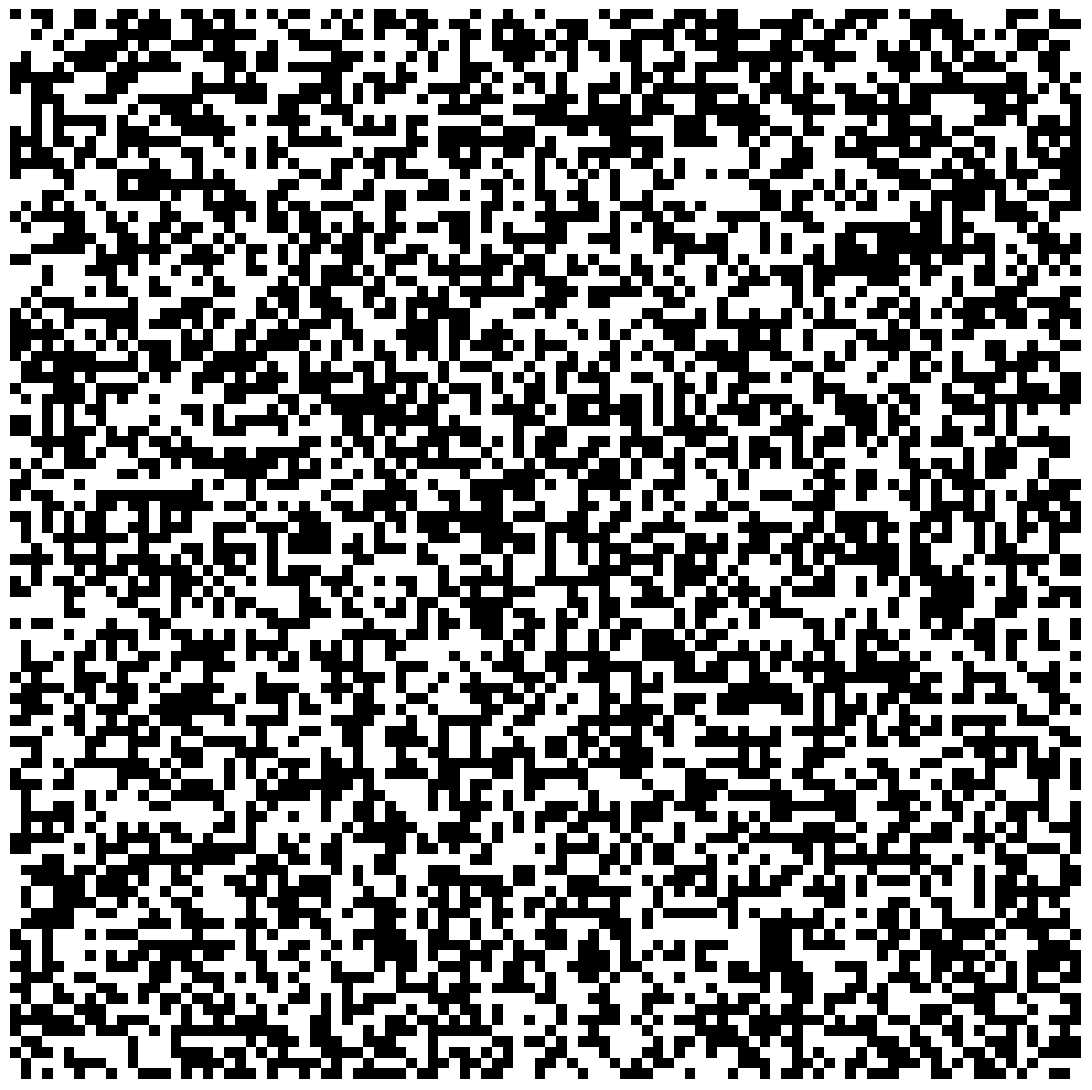
\includegraphics[width=0.65\textwidth]{Figures/verification_melted_lattice.png}
\caption{``Melted'' state of originally ordered lattice at low coldness (high temperature).
Disorder dominates even though $A$-$A$ and $B$-$B$ are energetically favorable relative to $A-B$.}
\label{fig:melted_lattice}
\end{figure}

Second, we show that the method produces highly ordered results when the system is cold and $w_{AB} > w_{AA},w_{BB}$, even if the initial state is entirely random.
Again $d=2 (z=4)$, $L=100$, $x=0.5$,  $w_{AA}=-1$ eV, $w_{BB} = -1$ eV, and $w_{AB} = -0.5$, however now $\beta = 100$ eV$^{-1}$ ($T=116$ K). meaning that the system should energetically prefer minimizing $A$-$B$ contacts.
At such a low temperature, the system should attempt to minmize $A$-$B$ contacts, since they are the least energetically favorable (most positive).
Indeed, even when the lattice is initially random, the system tends to an ordered state with long range order, as shown in Figure \ref{fig:frozen_lattice}
Again, the accompanying convergence plot (Figure \ref{fig:frozen_convergence}) is in the Appendix, and shows 

\begin{figure}[h!]
\centering
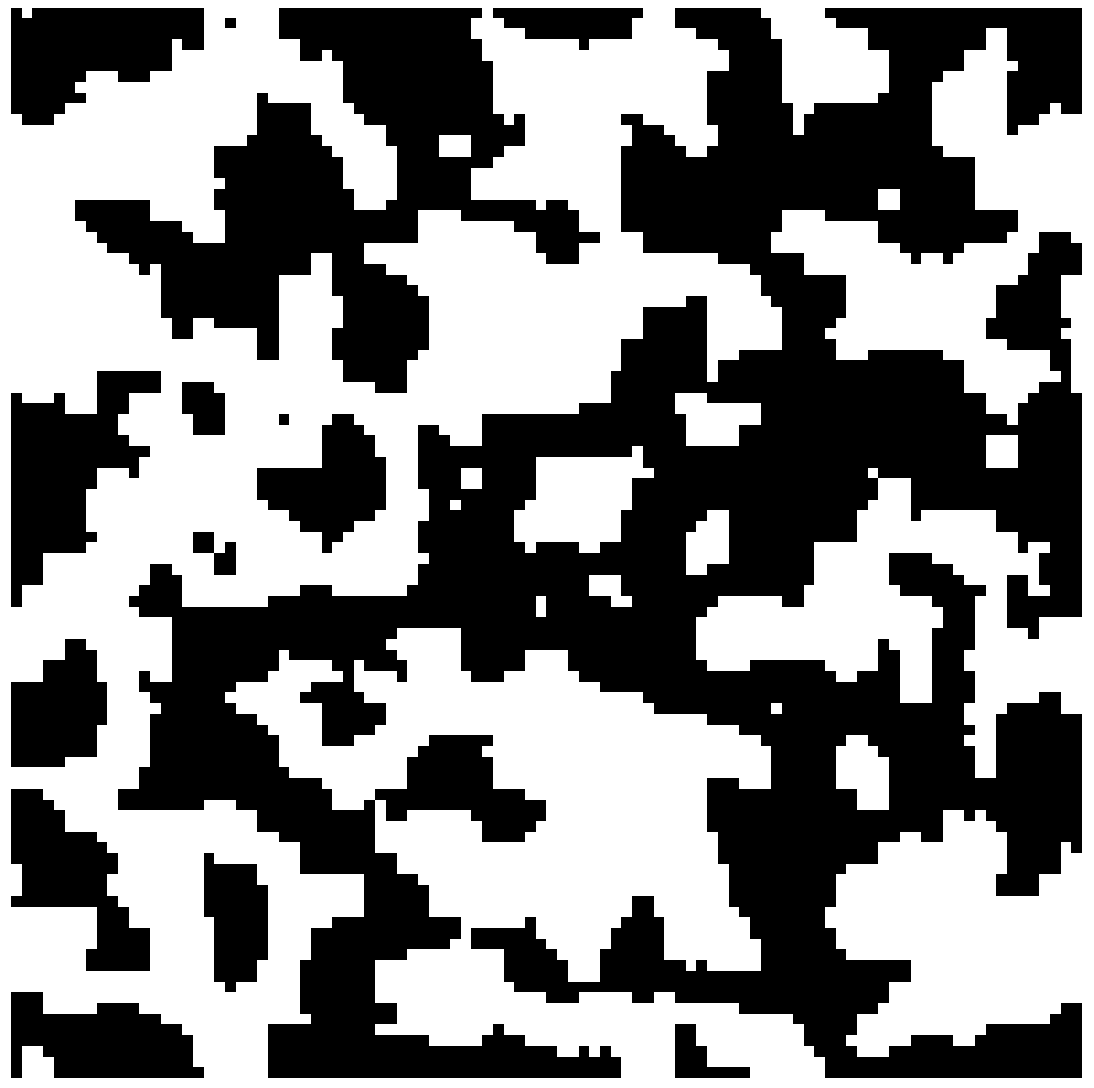
\includegraphics[width=0.65\textwidth]{Figures/verification_frozen_lattice.png}
\caption{``Frozen'' state of originally random lattice at low coldness (high temperature).
Order dominates, following physical intuition.}
\label{fig:frozen_lattice}
\end{figure}

\subsection{One dimensional trends in free parameters}
To visualize the dependence of $\hat{m}_{AB}$ on the system parameters $z,x,\beta,w_{AA},w_{BB},w_{AB}$, we perform plots meshing over each of these parameters, while holding the others constant at $z=4$ ($d = 2$), $x = 0.5$, $\beta = 38.7$ eV$^{-1}$ ($T = 300$ K), $w_{AA} = -1.0$ eV, $w_{BB} = 1.0$ eV, $w_{AB} = -0.5$ eV.
These plots are collected in Figures \ref{fig:m_AB_hat_versus_z} - \ref{fig:m_AB_hat_versus_w_AB}, respectively.

Figure \ref{fig:m_AB_hat_versus_z} shows a nearly linear relationship between $z$ and $\hat{m}_{AB}$ for the test system. \footnote{It is difficult to ascertain the functional form of the dependence with only three points, but this dependence is expected to be linear, as we justify in the next section.} 
Figure \ref{fig:m_AB_hat_versus_x} shows a nonlinear relationship between $z$ and $\hat{m}_{AB}$ for the test system.
Figure \ref{fig:m_AB_hat_versus_beta} displays a sharp transition between just above $\beta = 1$. For very cold systems this configuration minimizes $B$-$B$ interactions in favor of $A$-$B$ interactions, with less preference for $A$-$B$ interactions in system with low coldness (high temperature).
Figure \ref{fig:m_AB_hat_versus_w_AA} shows almost no dependence of $m_{AB}$ on $w_{AA}$, with the present variations likely due to noise.
Figure \ref{fig:m_AB_hat_versus_w_BB} shows another distinct transition-like structure centered around $w_{BB}=0$ eV.
By symmetry it is therefore likely that a similar dependence exists on $w_{AA}$, but perhaps it is not visible due to the asymmetry in the default values of the $w_{XY}$s.
Finally, Figure \ref{fig:m_AB_hat_versus_w_AB} shows a clear transition-like dependence of $\hat{m}_{AB}$ on $w_{AB}$.

\begin{figure}[h!]
\centering
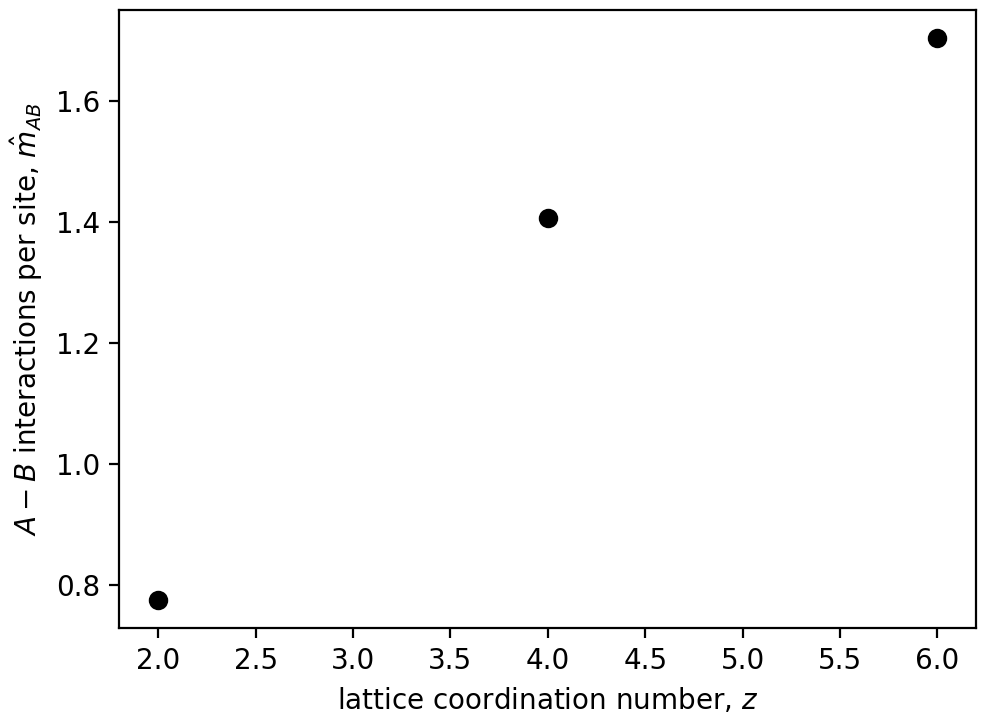
\includegraphics[width=0.65\textwidth]{Figures/m_AB_hat_versus_z.png}
\caption{Number of $A$-$B$ interactions per site versus lattice coordination number $z$.}
\label{fig:m_AB_hat_versus_z}
\end{figure}

\begin{figure}[h!]
\centering
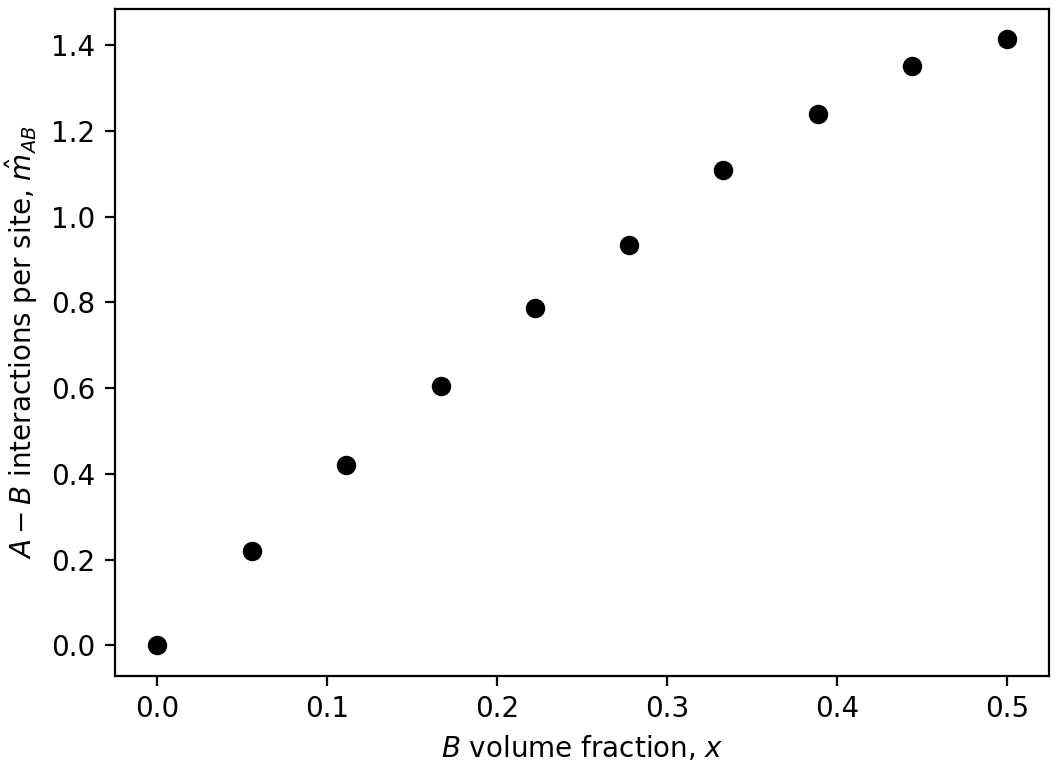
\includegraphics[width=0.70\textwidth]{Figures/m_AB_hat_versus_x.png}
\caption{Number of $A$-$B$ interactions per site versus $B$ volume fraction $x$.}
\label{fig:m_AB_hat_versus_x}
\end{figure}

\begin{figure}[h!]
\centering
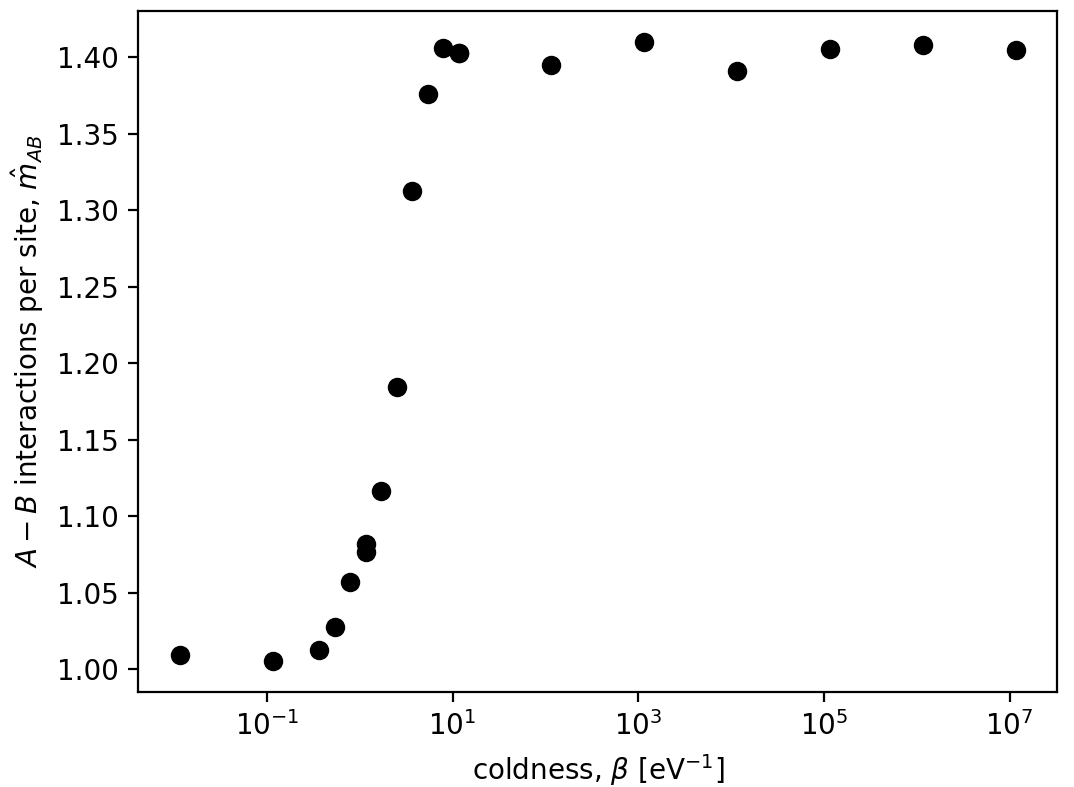
\includegraphics[width=0.67\textwidth]{Figures/m_AB_hat_versus_beta.png}
\caption{Number of $A$-$B$ interactions per site versus coldness $\beta = \frac{1}{k_B T}$.}
\label{fig:m_AB_hat_versus_beta}
\end{figure}

\begin{figure}[h!]
\centering
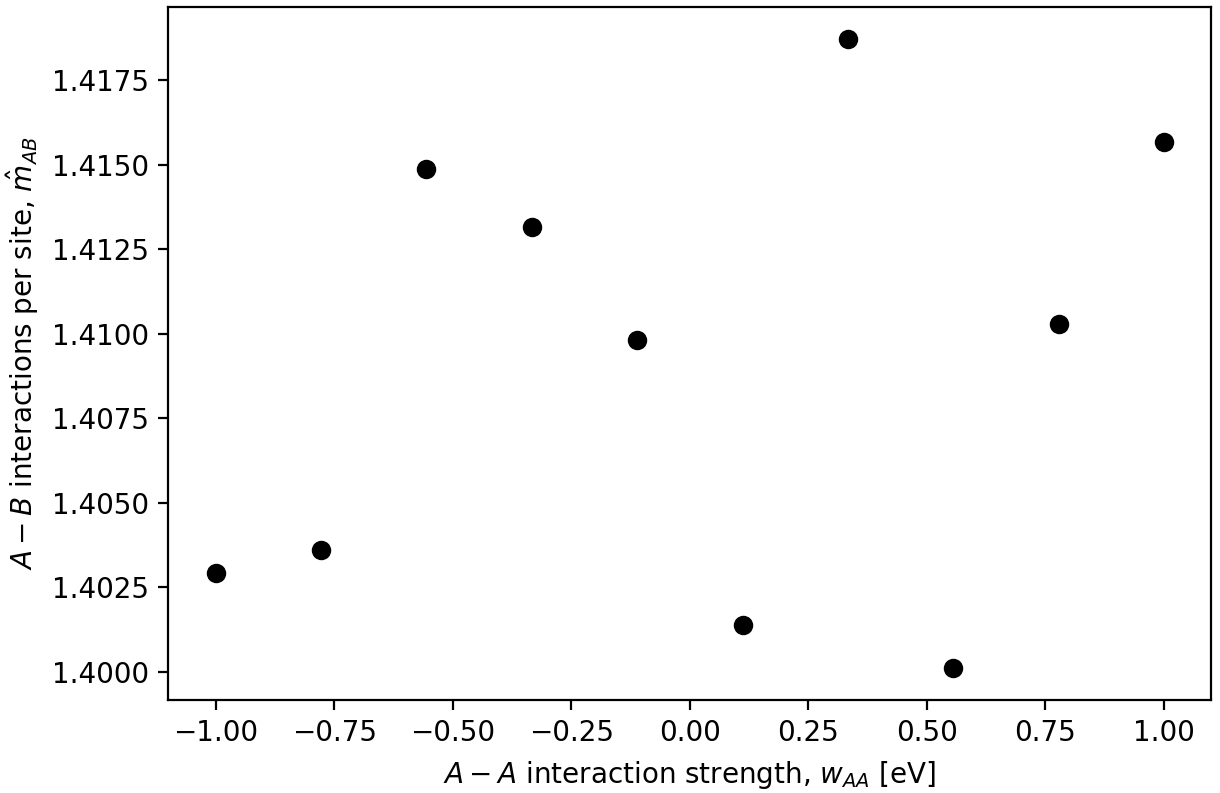
\includegraphics[width=0.70\textwidth]{Figures/m_AB_hat_versus_w_AA.png}
\caption{Number of $A$-$B$ interactions per site versus $A$-$A$ interaction strength $w_{AA}$.}
\label{fig:m_AB_hat_versus_w_AA}
\end{figure}

\begin{figure}[h!]
\centering
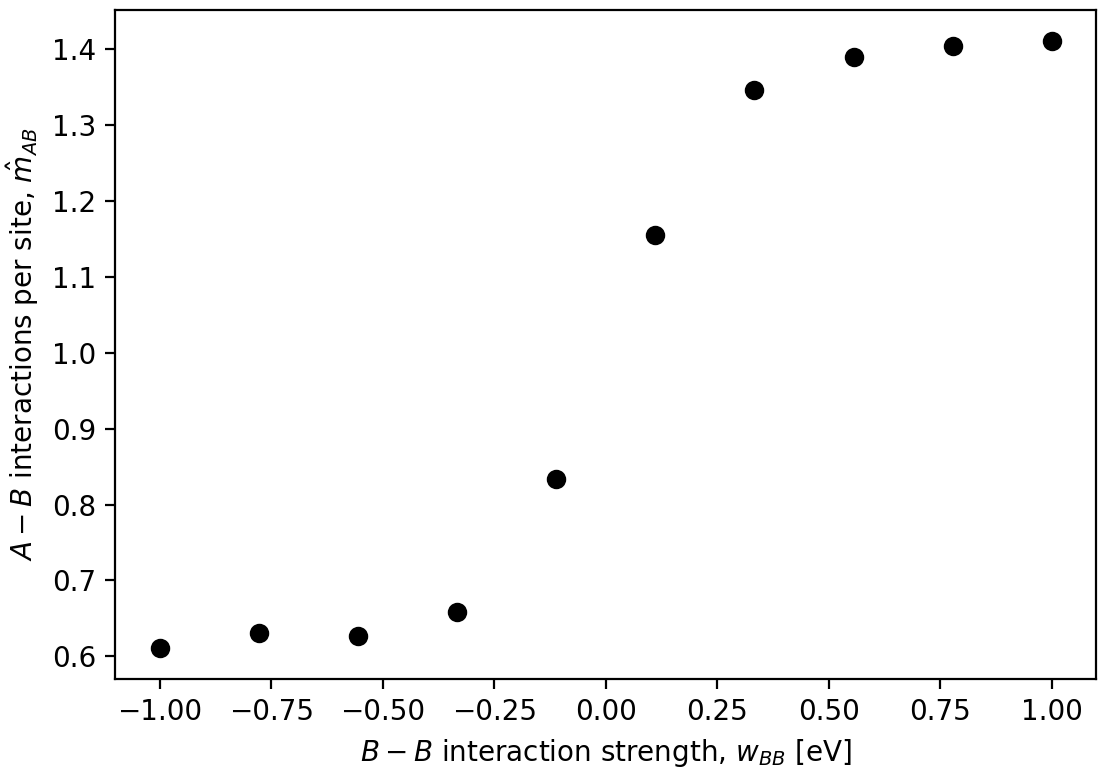
\includegraphics[width=0.70\textwidth]{Figures/m_AB_hat_versus_w_BB.png}
\caption{Number of $A$-$B$ interactions per site versus $B$-$B$ interaction strength $w_{BB}$.}
\label{fig:m_AB_hat_versus_w_BB}
\end{figure}

\begin{figure}[h!]
\centering
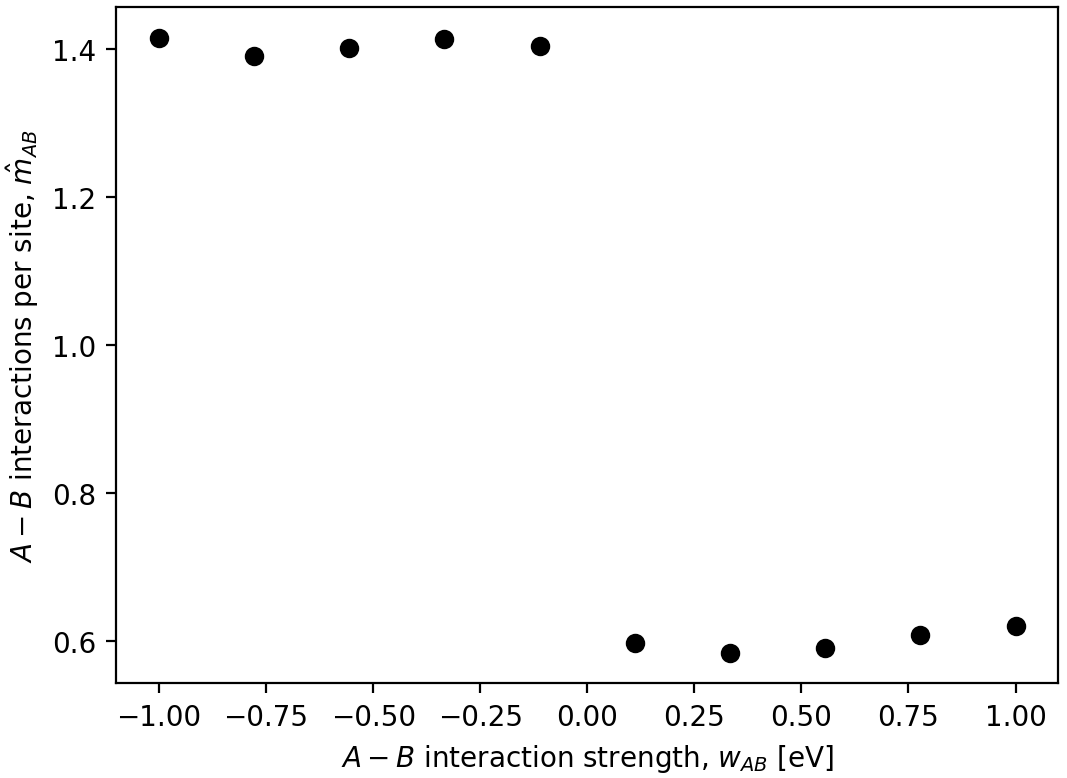
\includegraphics[width=0.70\textwidth]{Figures/m_AB_hat_versus_w_AB.png}
\caption{Number of $A$-$B$ interactions per site versus $A$-$B$ interaction strength $w_{AB}$.}
\label{fig:m_AB_hat_versus_w_AB}
\end{figure}

\subsection{Solutions at selected parameter points}
The MALM implementation was finally used to generate a data set of points occupying subset of the parameters space over $z,L,x,\beta,w_{AA},w_{BB},w_{AB}$.
Given that the goal of such microscale and nanoscale simulations the inclusion of the number of of sites per lattice edge $L$ may seem like an odd choice of free parameter (and indeed it does not appear in the final data set).
However, smaller systems converge much more quickly since the configuration space is smaller, and therefore having multiple equivalent configurations with a variety of system sizes is intended to provide a balance between the exactly converged systems and the thermodynamic limit.
Also, note that all treatment of the model is done on a per-site basis, so the extra dimension introduced by $L$ is eliminated by normalization by $N$.

Table \ref{tbl:param_ranges} lists the possible ranges for each of the seven parameters used when generating sample data points.
The spatial dimension $d$ covers all common model dimensions for physical systems.
As mentioned above, the side lattice side length $L$ was chosen to mix small lattices that almost certainly converge to the proper energy with larger lattices at the edge of the computational limit that better represent real physical systems.
The $B$ volume fraction $x$ only varies between 0 and 0.5 because the system is symmetric under a relabeling of $A \leftrightarrow B, w_AA \leftrightarrow w_BB$.
The interactions strengths were chosen with reference to real physical systems like water with hydrogen bonds of strength -0.24 eV and liquid argon (a common molecular dynamics model system) with equilibrium interaction -0.01 eV \cite{water} \cite{argon}.
The range for temperature $T$ goes from absolute zero to one million Kelvin, which is approximately the point at which the thermal energy scale $k_B T$ is equal to that of the the interaction energy scale defined by $w_XY$.

The points to at which MALM was used to solve the system include all $2^7$ vertices of the hypercube defined by the extreme values of the parameters in Table \ref{tbl:param_ranges}, in addition to 1000 random points from the interior of the hypercube.
At each of these 1128 points, the internal energy $U$ was computed using MALM, with termination at $200 \times 10^3$ iterations or $\hat{S}_{\bar{U}} < 5 \times 10^{-5}$ (whichever came first).
For all points the lattice was initialized as a random lattice of the specified $B$ volume fraction $x$.
This raw data consisting of points like $(d,x,L,T,w_{AA},w_{BB},w_{AB},U)$, was then processed to generate corresponding points $(z,x,\beta,w_{AA},w_{BB},w_{AB},\hat{m}_{AB})$.

\begin{center}
\begin{tabular}{c | l | l | l} 
    \hline
    Parameter & Possible Values & Grid spacing & Units \\  \hline
    $d$ & $\mathbb{Z} \in \{1,2,3\}$ & discrete & not applicable \\ \hline
    $L$ & $\mathbb{Z} \in [5,100]$ & discrete & not applicable \\ \hline
    $x$ & $\mathbb{R} \in [0.0,0.5)$ & linear & not applicable \\ \hline
    $T$ & $\mathbb{R} \in [1.0 \times 10^{-3},1.0 \times 10^6]$ & logarithmic & K \\ \hline
    $w_{AA}$ & $\mathbb{R} \in [-1.0, 1.0]$ & linear & eV \\ \hline
    $w_{BB}$ & $\mathbb{R} \in [-1.0, 1.0]$ & linear & eV \\ \hline
    $w_{AB}$ & $\mathbb{R} \in [-1.0, 1.0]$ & linear & eV \\
    \label{tbl:param_ranges}
\end{tabular}
\end{center}


\section{Model Construction}
The model function $f_{\hat{m}_{AB}}$ contributes to the internal energy per site as

We now turn our attention to using the data set from the previous section to create a semi-emperical model for the lattice mixture internal energy per site.
We work in terms of a function $f_{\hat{m}_{AB}}$ intended to approximate $\hat{m}_{AB}$, which contributes to the internal energy per site as
\begin{align}
    \hat{U} = \frac{z}{2} \left( (1-x) w_{AA} + x w_{BB} \right) +
    f_{\hat{m}_{AB}} \left( w_{AB} - \frac{w_{AA} + w_{BB}}{2} \right)
    \label{eqn:model_U}
\end{align}
We seek the optimal model parameters $\mathbf{v}^*$ for $f_{\hat{m}_{AB}}(\mathbf{p},\mathbf{v})$, where $\mathbf{p}$ is  parameter point (including $z,x,\beta$,etc.) and $\mathbf{v}$ is the vector of model parameters.
The optimal model parameters sastify the optimality conditions of the nonlinear least squares problem
\begin{align}
\phi(\mathbf{v}) = \mathbf{r}(\mathbf{v})^T \mathbf{r}(\mathbf{v}),
\quad\quad r_i = \hat{m}_{AB}^{(i)} - f_{\hat{m}_{AB}}(\mathbf{p}^{(i)},\mathbf{v})
\end{align}
where $i$ denotes the $i$ data point of the data/sample set (consisting of pairs $(\mathbf{p},\hat{m}_{AB})$, and ranges from one to the number of sampled points.
Of course, multiple model functions are possible, and we compare a few alternatives, including the function corresponding to the Bragg-Williams approximation.

\subsection{Constraints on the modeling function}
Although many model functions forms are possible, not all are physical.
Feasible model functions for $\hat{m}_{AB}$ must satisfy a number of properties, including symmetry in the some of th parameters, have certain certain limiting behaviors, and so on, which we now attempt to state in mathematical detail.

First, since the labelling of $A$ and $B$ is just a notational convention, the equation of $w_{AB}$ should be invariant under respective exchanges $(x,w_AA,w_BB) \longleftrightarrow (1-x,w_{BB},w_{AA})$.
Observe that the rest of the formula for $\hat{U}$ in Equation \ref{eqn:model_U} satisfies this symmetry automatically, as does the so-called Bragg-Williams model function for $\hat{m}_{AB}$
\begin{align}
    f_{\hat{m}_{AB},BW} = z (1-x) x.
    \label{eqn:BW_model_function}
\end{align}

In the low coldness (high temperature) macrostates occupy all microstates with equal probability, giving rise to a random lattice (with fixed $B$ volume fraction $x$, of course) in equilibrium.
Consequently, such a random lattice is exactly the assumption of the Bragg-Williams approximation.
Therefore, in the low coldness limit our model function must reduce to the Bragg-Williams model function
\begin{align}
    \lim_{\beta \rightarrow 0} f_{\hat{m}_{AB}} = z (1-x) x.
\end{align}

Additionally, we assert that $f_{\hat{m}_{AB}}$ should be linearly dependent on $z$.
The other term in Equation \ref{eqn:model_U} and the Bragg-Williams model function both obey this dependence.
Furthermore, such dependence has a sensible heuristic argument.
Since $\hat{m}_AB$ counts interactions ``per-site'', it should be strictly proportional to the coordination number $z$ of a single site.
This is essentially equivalent to assuming occupation statistics are independent of the spatial dimension of the lattice, which is a reasonable first approximation.
Figure \ref{fig:m_AB_hat_versus_z} attempts to justify this assertion numerically, but it is difficult to extract the exact dependence with only three points.
Suprisingly, $\hat{m}_{AB}$ appears to be at least weakly nonlinear with $z$, which does not strictly conform to the linear assumption.

Lastly, we note that Figures \ref{fig:m_AB_hat_versus_beta} - \ref{fig:m_AB_hat_versus_w_AB} justify the exististence of some sort of Fermi-function-like behavior involving $\beta,w_{AA},w_{BB},w_{AB}$.
Of course of model function must also have the right units, which in our case is unitless, since the model function multiplies a term with units of energy in \ref{eqn:model_U}.

\subsection{Model functions}
[check that $m_AB$ is not off by factor of 2, etc.]

\begin{align}
    f_{\hat{m}_{AB},1} = 
    \frac{1}{1 + exp\left(\beta \left(w_{AB} - \frac{w_{AA} + w_{BB}}{2}\right) \right)}
    z (1-x) x
\end{align}


\subsection{Model results}

\section{Conclusion}




\clearpage
\section{Appendix}
\subsection{Permitted swaps}
Each Monte Carlo step proposes an exchange between two sites in the lattice.
Should each exchange propose swaps between two truly random lattice sites (possibly of the same type), or should each swap be forced to exchange lattice sites of different types.
Of course, swapping two sites of the same type will not change the internal energy, but how does the choice of permitted swaps affect convergence rate and average energy?
Figure \ref{fig:swap} below shows how convergence (in terms of number of Monte Carlo steps) differs for an example case.
One can see that while both choice result in the same mean energy, restricting every swap to exchange sites of different types has multiple advantages.
First, the ``transient'' or ``relaxation'' time (where the energy moves toward the equilibrium value) is about half the length, and the same error tolerance is achieved in about 70\% as many steps.
The effect of this choice will be more exaggerated for extremely low and  high volume fractions $x$, where the ``swap any two'' scheme has a high probability of selecting a pair of the same type ($a_i = b_j$), whose exchange will not affect the internal energy.
In that sense, the figure below gives the ``swap any two'' scheme the best chance for success, and it is still found to be less efficient.

\begin{figure}[h!]
\centering
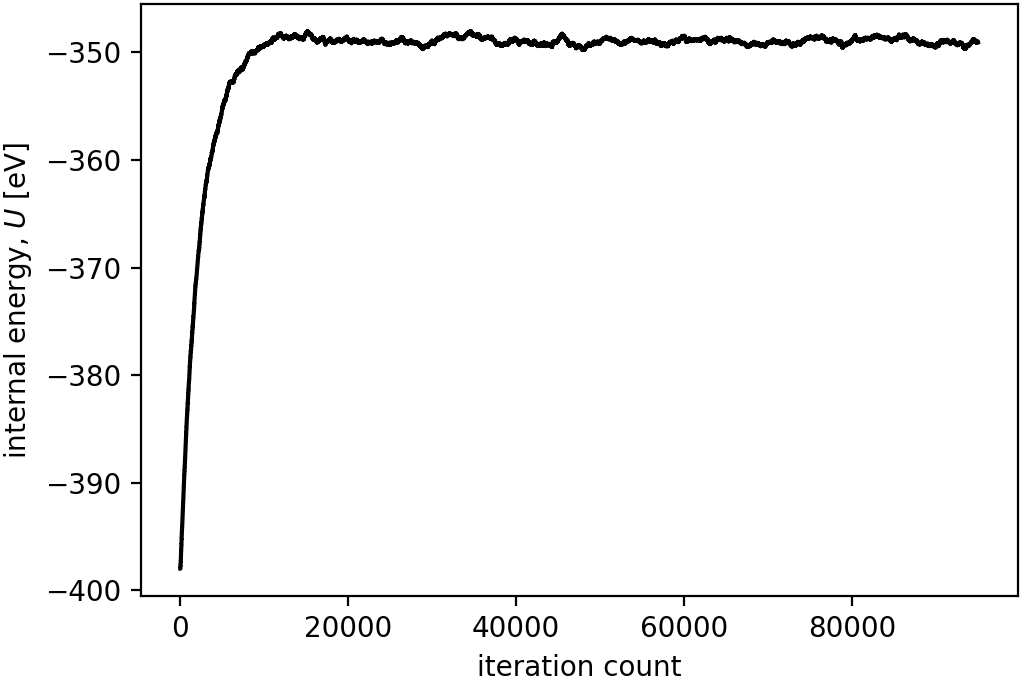
\includegraphics[width=0.65\textwidth]{Figures/swap_any_two_convergence.png}
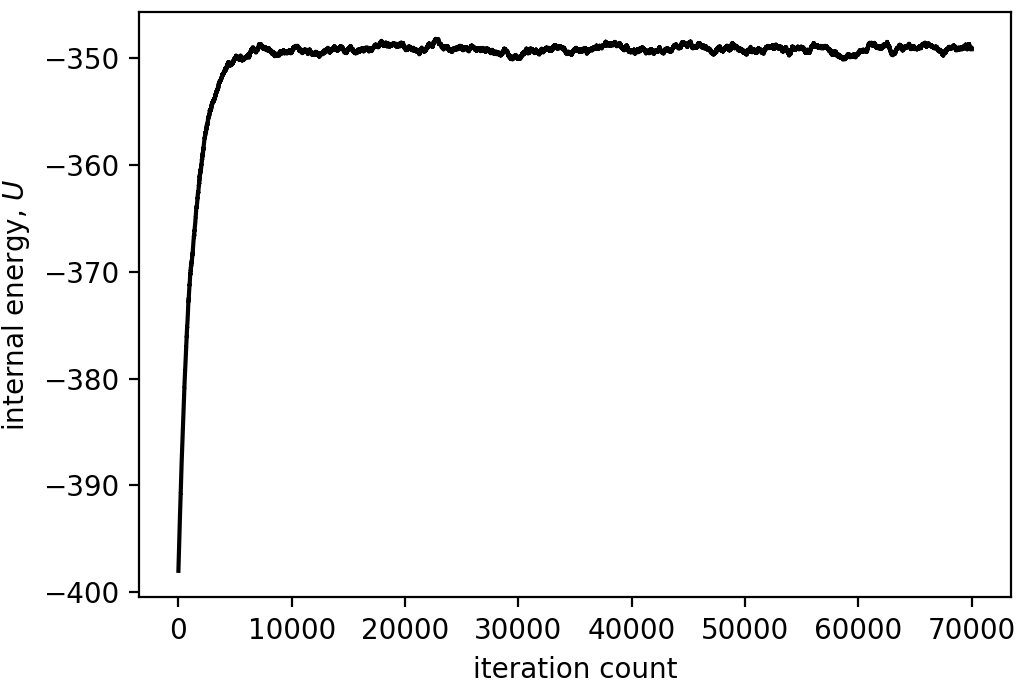
\includegraphics[width=0.65\textwidth]{Figures/swap_A_B_only_convergence.png}
\caption{Internal energy versus iteration with $L=100$, $d=2$, $x=0.5$, $\beta=0.1$, $w_{AA}=w_{AB}=-10 \times 10^{-3},w_{BB} = -30 \times 10^{-3}$ eV; both simulations were run until the percentage error in the mean energy was less than 0.005\%.
The upper figure is when swaps may exchange any two sites (independent of their types), while the bottom figure permits exchanges only between A and B sites.}
\label{fig:swap}
\end{figure}

\subsection{Convergence of verification runs}

\begin{figure}[h!]
\centering
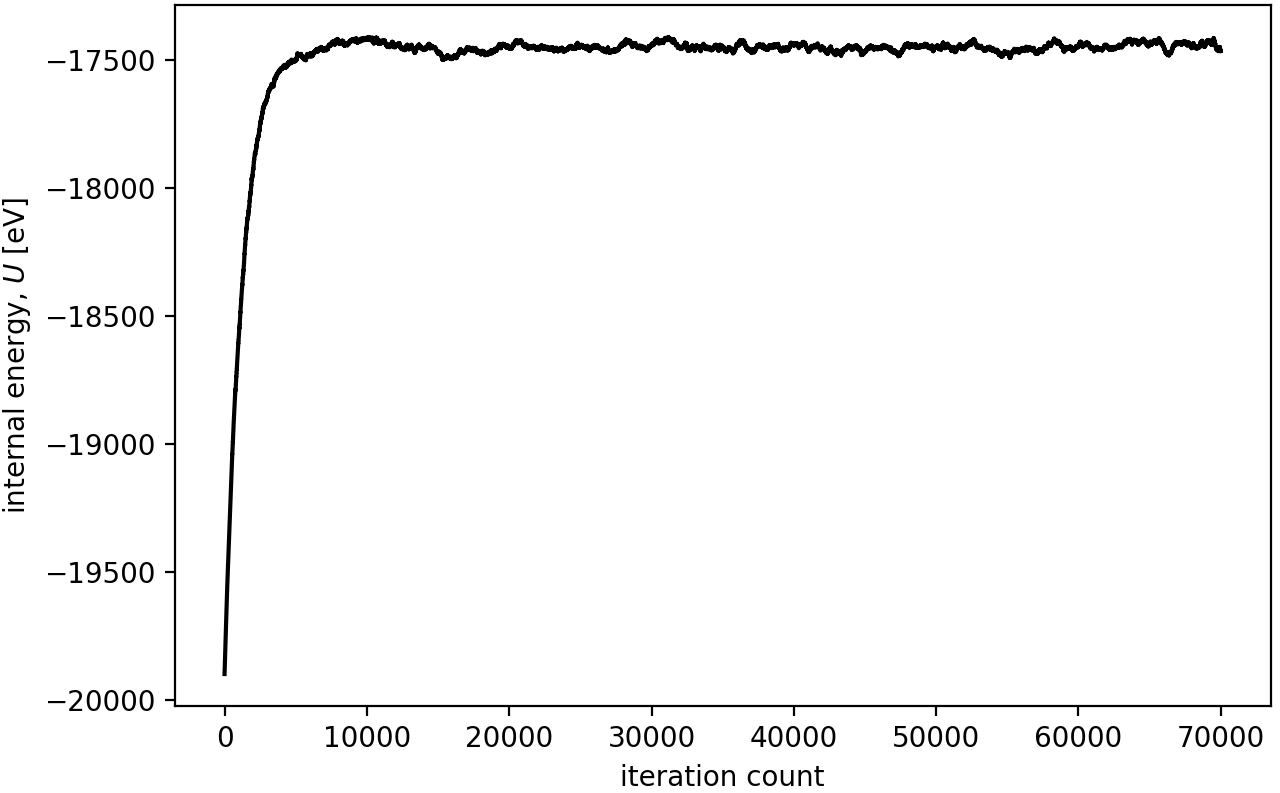
\includegraphics[width=0.80\textwidth]{Figures/verification_melted_convergence.png}
\caption{Energetic convergence to the equilibrium random ``melted'' state of an originally ordered lattice at low coldness (high temperature).
Disorder dominates even though $A$-$A$ and $B$-$B$ are energetically favorable relative to $A$-$B$, and the system starts at in a configuration that minimizes $A$-$B$ contacts.
The larger variations after convergence characterize the low coldness (high temperature).}
\label{fig:melted_convergence}
\end{figure}

\begin{figure}[h!]
\centering
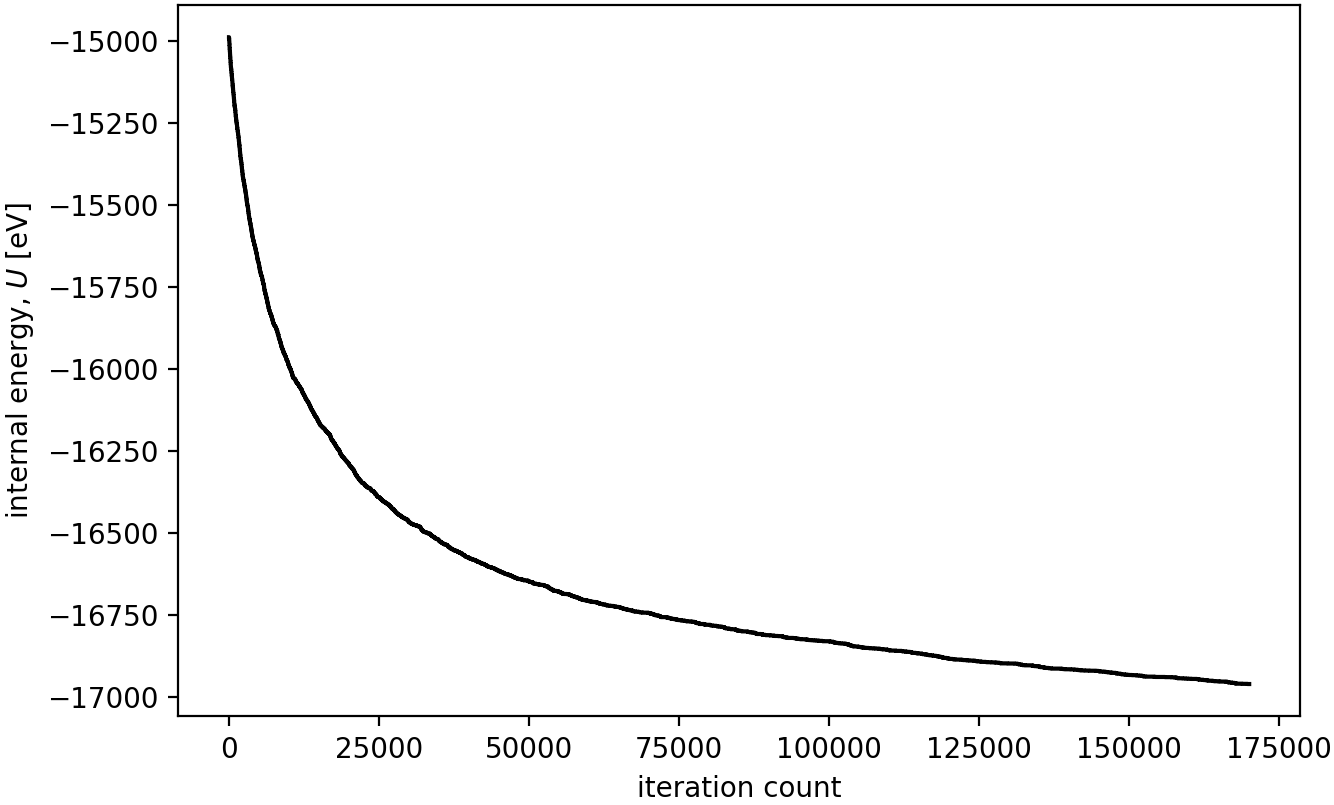
\includegraphics[width=0.80\textwidth]{Figures/verification_frozen_convergence.png}
\caption{Energetic convergence to the equilibrium random ``frozen'' state of an originally random lattice at high coldness (low temperature).
Long range order and structure dominates, driven by energy minimization to reduce the total $A-B$ surface area.
The low variations throughout characterize the high coldness (lower temperature), as the system nearly primarily minimizes energy from step to step.}
\label{fig:frozen_convergence}
\end{figure}


\clearpage
\bibliography{references.bib}
References (USE BIBTEX THOUGH)


\end{document}

